\documentclass{article}
\iffalse
This file is protected by Copyright. Please refer to the COPYRIGHT file
distributed with this source distribution.

This file is part of OpenCPI <http://www.opencpi.org>

OpenCPI is free software: you can redistribute it and/or modify it under the
terms of the GNU Lesser General Public License as published by the Free Software
Foundation, either version 3 of the License, or (at your option) any later
version.

OpenCPI is distributed in the hope that it will be useful, but WITHOUT ANY
WARRANTY; without even the implied warranty of MERCHANTABILITY or FITNESS FOR A
PARTICULAR PURPOSE. See the GNU Lesser General Public License for more details.

You should have received a copy of the GNU Lesser General Public License along
with this program. If not, see <http://www.gnu.org/licenses/>.
\fi

% TODO: Version numbers?
\usepackage{graphicx}
\graphicspath{ {figures/} }
\usepackage{fancyhdr}
\usepackage{colortbl}
\usepackage[margin=.75in]{geometry}
\usepackage{hyperref}
\usepackage{listings}
\pagestyle{fancy}
\lhead{Board Support Package Documentation}
\rhead{ANGRYVIPER Team}
\renewcommand{\headrulewidth}{0pt}
\newcommand{\shellcmd}[1]{\texttt{\$ #1\\}}
\newcommand{\terminaloutput}[1]{\texttt{#1}}
\definecolor{blue}{rgb}{.5,1,1}
\definecolor{drkgreen}{rgb}{0,.6,0}
\begin{document}
\section*{ML605 Hardware Setup}
\subsection*{Prerequisites}
\begin{itemize}
\item A valid development system which has OpenCPI and Xilinx installed. These instructions were performed using Xilinx ISE 14.7. Note that Xilinx cable drivers must be installed for OpenCPI's loadFlash command to work properly.
\end{itemize}
\subsection*{Hardware Description}
The ML605 is the PCI-Express development board for Virtex 6. It can be purchased directly from Xilinx or a distributor. Xilinx's URL for the board containing user guides and reference manuals can be found here:\par\bigskip
​\url{http://www.xilinx.com/products/boards-and-kits/ek-v6-ml605-g.html#documentation}\par\bigskip
\noindent  There is one version of the board. The below table contains platform name and part number for the development board.\par\bigskip
\begin{tabular}{|c|c|c|}
\hline
\rowcolor{blue}
OpenCPI Platform Name & Xilinx Kit Part Number & FPGA Part Number \\
\hline
ml605 & EK-V6-ML605-G & XC6VLX240T-1FFG1156 \\
\hline
\end{tabular}\par\bigskip
\subsection*{Setup Overview}
To use this board within OpenCPI, the board must be configured to load the FPGA with an OpenCPI bitstream upon power up. There is flash memory on the board which can be loaded with a bitstream to load the FPGA on power up. The process for loading this flash is:
\begin{enumerate}
\item Configure the board to boot from flash memory and the PCIe lane size.
\item Install board into OpenCPI development host.
\item Verify JTAG connection using OpenCPI script.
\item Run OpenCPI loadFlash script.
\item Verify that the ML605 is configured with a OpenCPI bitstream.
\item Modification of /opt/opencpi/system.xml
\end{enumerate}
 Details for implementing this procedure can be found in the sections below.
\pagebreak
\subsubsection*{Configure the board to boot from flash memory and the PCIe lane size}
For more information about configuring the ML605, reference Xilinx ML605 Hardware User Guide, UG534.pdf (v1.8) October 2, 2012.
\begin{enumerate}
\item The S2 DIP switch is a multi-purpose selector switch. It controls the state of the FPGA's configuration mode pins and must be set for ``Slave SelectMAP Platform Flash XL'' to boot from flash memory. Below is a picture of the S2 DIP switch with the expected setting:
\\\smallskip
\begin{center}
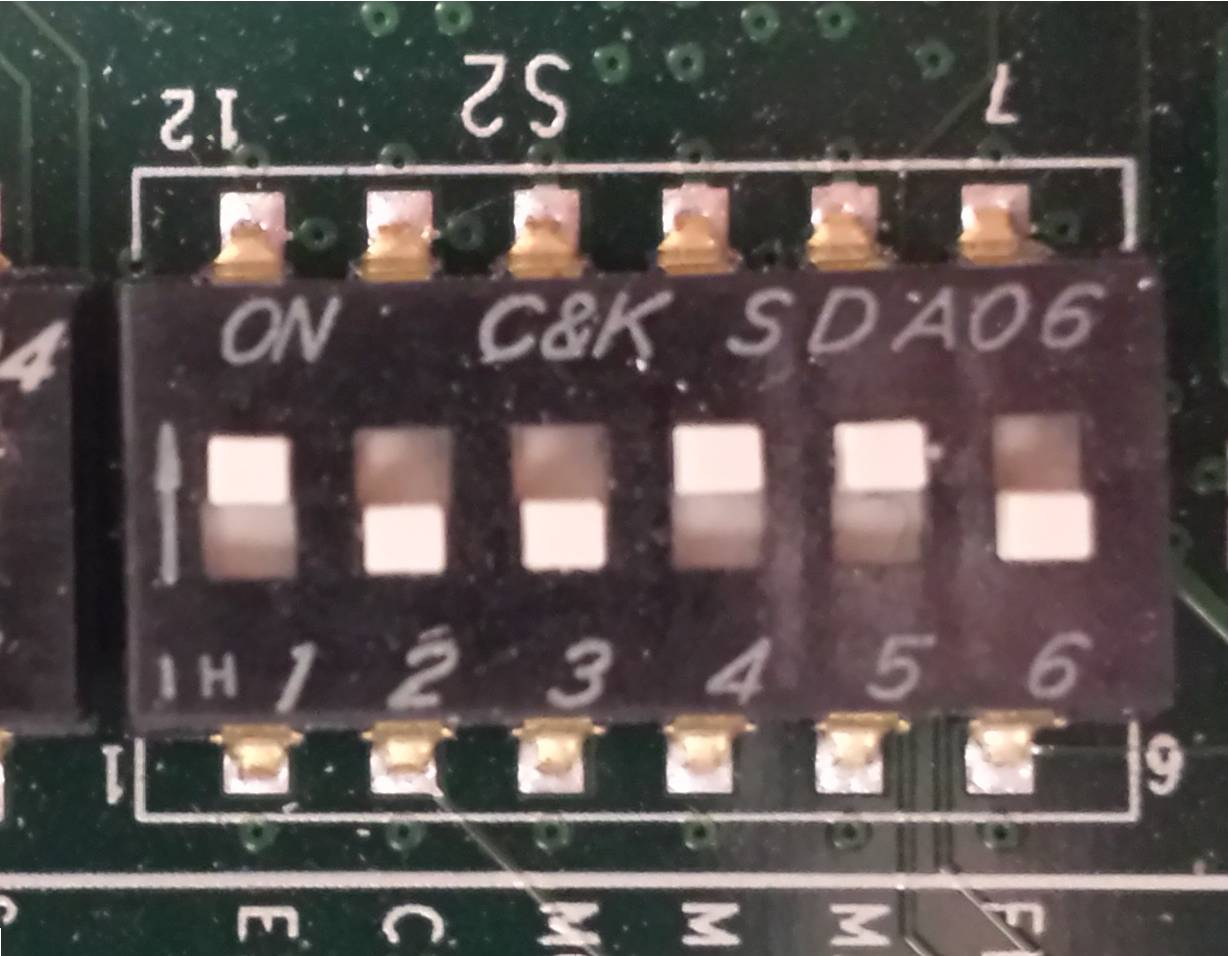
\includegraphics[scale=0.20]{ML605_S2.jpg}\par\smallskip
 The table below contains the expected S2 DIP switch settings.\par\smallskip
\begin{tabular}{|c|c|c|c|c|c|}
\hline
\rowcolor{blue}
S2.1 & S2.2 & S2.3 & S2.4 & S2.5 & S2.6 \\
\hline
on & off & off & on & on & don't care \\
\hline
\end{tabular}
\end{center}\par\bigskip
\item The J42 configures the board to support 4x PCIe lanes. Below is a picture of J42 with a 100mil shunt installed in the correct position.
\begin{center}
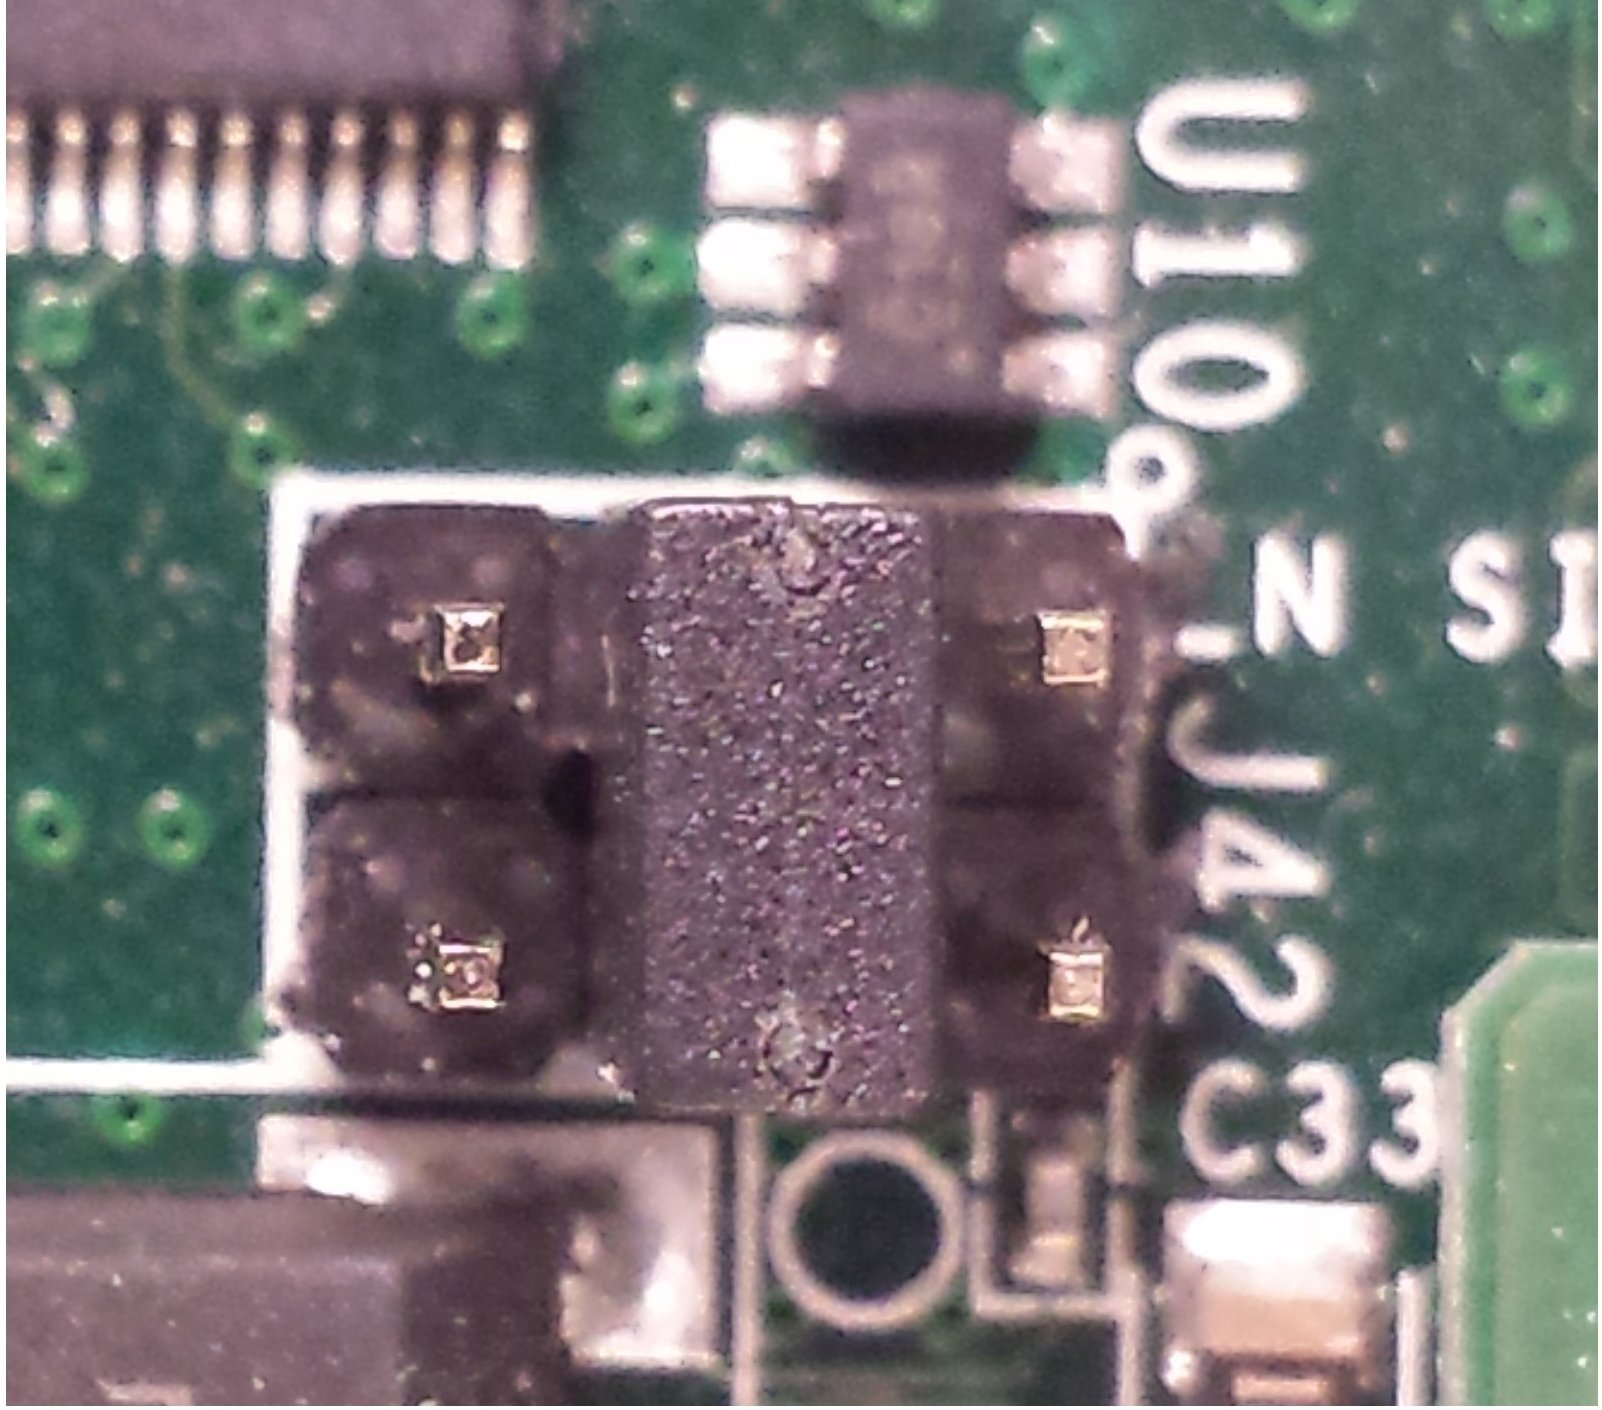
\includegraphics[scale=0.15]{ML605_J42.jpg}\par\bigskip
\end{center}
\end{enumerate}
\pagebreak
\subsubsection*{Install board into OpenCPI development host}
\begin{enumerate}
\item Power off the development host.
\item Following anti-static best practices, insert the ML605 into a compatible PCIe slot.
\item Attach the USB cable between the ML605 JTAG port and a host USB port.
\item With the AUX power supply unplugged (powered OFF), attach the AUX power cable to the ML605 AUX power-in connector.
\item Power ON the AUX power supply by plugging it an A/C outlet. (at this point the development host is still OFF)
\item Locate the SW2 on the ML605, and switch it to the ON position, i.e, slide away from the AUX power-in connector. The board will power up, but the development host is not powered on.
\item Power ON the development host.
\end{enumerate}
\subsubsection*{Verify JTAG connection using OpenCPI script}
\begin{enumerate}
\item Enter a terminal and source the OpenCPI environment for x86.
\item Run the following script to test the JTAG connection: opencpi/hdl/scripts/probeJtag
\end{enumerate}
\par\smallskip
\noindent An example of the output is shown below:\par\smallskip
\noindent\terminaloutput{==== Probing for Altera JTAG ports:\\
Altera directory set by (OCPI\_ALTERA\_TOOLS\_DIR) does not exist.\\==== Probing for Xilinx JTAG ports:\\Discovered ports are: usb21\\Trying port usb21...  ESN is 000013C8121101\\Part at position 1 on is xccace\\Part at position 2 on is xc6vlx240t.}\par\bigskip
\noindent For the purposes of this guide, ignore any messages related to Altera.\par\smallskip
\noindent If the output doesn't look like this, refer Xilinx documentation to ensure the JTAG cable is correctly installed and operational.\par\smallskip
\subsubsection*{Run OpenCPI loadFlash script}
\begin{enumerate}
\item The loadFlash script is located at opencpi/tools/cdk/scripts. You must pass it a pre-built ML605 .bitz file generated by OpenCPI and the serial number (in hex) of the JTAG cable from probeJtag script above. This step with take approximately 10 minutes to complete.\par\smallskip
\noindent{\bf ML605 syntax}\par
\noindent\shellcmd{loadFlash ml605 <OpenCPI Bitstream File> <JTAG\_CABLE\_SERIAL\_NUMBER>}\par\smallskip
\noindent{\bf Example output}\par
\noindent\terminaloutput{\$ loadFlash ml605 hdl/platforms/ml605/testbias\_ml605\_base.bitz 000013C8121101\\
Loading the flash memory on the ml605 platform attached to the JTAG pod with ESN 000013C8121101\\
Loading from file: hdl/platforms/ml605/testbias\_ml605\_base.bitz\\
Looking for the Xilinx USB port corresponding to JTAG Pod ESN 000013C8121101.\\
Discovered ports are: usb21\\
Trying usb21... ESN is: 000013C8121101\\
Found ESN 000013C8121101 on usb21, using it.\\
The bitstream file "hdl/platforms/ml605/testbias\_ml605\_base.bitz" is compressed. Expanding it.\\
Bitstream file decompressed into "/tmp/ocpibitstream3100.bit"\\
Converting "/tmp/ocpibitstream3100.bit" to flash format in "/tmp/ocpibitstream3100.mcs" using xilinx promgen tool.\\
Executing command: /opt/Xilinx/14.5/ISE\_DS/ISE/bin/lin64/promgen -w -p mcs -c FF -x xcf128x -data\_width 16 -u 00000000 /tmp/ocpibitstream3100.bit\\
Conversion to flash file format succeeded. Starting flash programming.\\
This can take a while - 10-15 minutes. Starting at 09:57:27.\\ \\
real	11m55.080s\\
user	0m28.494s\\
sys	0m7.742s\\
Flash programming is complete. You must power-cycle the system to use it\\
Use the "ocpihdl search" command after power cycling to confirm success.}\par\bigskip
\item Once programming is complete, power cycle the system:
\item[i]Power OFF the host
\item[ii]Power cycle the ML605
\item[iii]Power ON the host
\end{enumerate}\par
\subsubsection*{Verify that the ML605 is configured with a OpenCPI bitstream}
\begin{enumerate}
\item Open a terminal window.
\item Execute the following Linux command to verify the presence of the ML605.\\
\noindent\shellcmd{ sudo lspci -vv\\ \\
03:00.0 RAM memory: Xilinx Corporation Device 4243 (rev 02)\\
Subsystem: Xilinx Corporation Device 0007\\
Control: I/O- Mem- BusMaster- SpecCycle- MemWINV- VGASnoop- ParErr- Stepping- SERR- FastB2B- DisINTx-\\
Status: Cap+ 66MHz- UDF- FastB2B- ParErr- DEVSEL=fast >TAbort- <TAbort- <MAbort- >SERR- <PERR- INTx-\\
	Interrupt: pin A routed to IRQ 11\\
	Region 0: Memory at e8000000 (32-bit, non-prefetchable) [disabled] [size=64M]\\
	Region 1: Memory at ec000000 (32-bit, non-prefetchable) [disabled] [size=1M]\\
	Capabilities: [40] Power Management version 3\\
		Flags: PMEClk- DSI- D1- D2- AuxCurrent=0mA PME(D0+,D1+,D2+,D3hot+,D3cold-)\\
		Status: D0 NoSoftRst+ PME-Enable- DSel=0 DScale=0 PME-\\
	Capabilities: [48] MSI: Enable- Count=1/1 Maskable- 64bit+\\
		Address: 0000000000000000  Data: 0000
	Capabilities: [60] Express (v2) Endpoint, MSI 01\\
		DevCap:	MaxPayload 512 bytes, PhantFunc 0, Latency L0s <64ns, L1 unlimited\\
			ExtTag- AttnBtn- AttnInd- PwrInd- RBE+ FLReset-\\
		DevCtl:	Report errors: Correctable- Non-Fatal- Fatal- Unsupported-\\
			RlxdOrd- ExtTag- PhantFunc- AuxPwr- NoSnoop+\\
			MaxPayload 256 bytes, MaxReadReq 256 bytes\\
		DevSta:	CorrErr- UncorrErr- FatalErr- UnsuppReq- AuxPwr- TransPend-\\
		LnkCap:	Port \#0, Speed 5GT/s, Width x4, ASPM L0s, Latency L0 unlimited, L1 unlimited\\
			ClockPM- Surprise- LLActRep- BwNot-\\
		LnkCtl:	ASPM Disabled; RCB 64 bytes Disabled- Retrain- CommClk-\\
			ExtSynch- ClockPM- AutWidDis- BWInt- AutBWInt-\\
		LnkSta:	Speed 5GT/s, Width x4, TrErr- Train- SlotClk- DLActive- BWMgmt- ABWMgmt-\\
		DevCap2: Completion Timeout: Range B, TimeoutDis-, LTR-, OBFF Not Supported\\
		DevCtl2: Completion Timeout: 50us to 50ms, TimeoutDis-, LTR-, OBFF Disabled\\
		LnkCtl2: Target Link Speed: 5GT/s, EnterCompliance- SpeedDis-\\
			 Transmit Margin: Normal Operating Range, EnterModifiedCompliance- ComplianceSOS-\\
			 Compliance De-emphasis: -6dB\\
		LnkSta2: Current De-emphasis Level: -3.5dB, EqualizationComplete-, EqualizationPhase1-
			 EqualizationPhase2-, EqualizationPhase3-, LinkEqualizationRequest-\\
	Capabilities: [100 v1] Device Serial Number 00-00-00-01-01-00-0a-35\\
	Kernel modules: windrvr6
		}\par\smallskip
\item In the terminal window, source the OpenCPI environment for x86.
\item Execute an OpenCPI utility which calls Xilinx iMPACT to scan JTAG for devices\smallskip
\noindent\terminaloutput{\\\$ probeJtag\\
==== Probing for Altera JTAG ports:\\
Altera directory (set by OCPI\_ALTERA\_TOOLS\_DIR) does not exist.\\
==== Probing for Xilinx JTAG ports:\\
Discovered ports are: usb21\\
Trying port usb21...  ESN is 000013C8121101\\
Part at position 1 on is xccace\\
Part at position 2 on is xc6vlx240t}\par\smallskip
\item Load the OpenCPI driver (requires sudo privileges):\smallskip
\noindent\terminaloutput{\\\$ ocpidriver load}
\item Execute an OpenCPI utility\smallskip
\noindent\terminaloutput{\\\$ ocpihdl search\\
OpenCPI HDL device found: 'PCI:0000:03:00.0': bitstream date Fri Jun 26 15:14:21 2015, platform "ml605", part "xc6vlx240t", UUID 8cd0a91e-1c37-11e5-8b5f-f30e2f82978a}
\item Perform a container check using ocpirun -C. The result should look like this:\smallskip
\noindent\terminaloutput{\\\$ ocpirun -C\\
Available containers:\\
 \#  Model\hspace{6ex} Platform\hspace{3ex}    OS\hspace{5ex}     OS Version\hspace{1ex}  Name\\
 0  rcc\hspace{9ex}   x86\_64\hspace{5ex}      linux\hspace{2ex}  c6\hspace{10ex}          rcc0\\
  1  hdl\hspace{9ex}   ml605\hspace{29ex}                          PCI:0000:03:00.0}\\
\end{enumerate}
\subsubsection*{Modification of /opt/opencpi/system.xml}
When multiple boards from same vendor are installed, and thus more than one JTAG USB, the OpenCPI load function (either explicit in "ocpihdl load" or implicit in 'ocpirun' needs to know which JTAG USB to use. The '/opt/opencpi/system.xml' file is used to map the PCI:* with JTAG USB serial number information. An example is shown below:\par\bigskip
\noindent\terminaloutput{<opencpi>\\
<container>\\
<hdl>\\
<device name="0000:03:00.0" esn="000013C8121101"/>\\
<device name="0000:08:00.0" esn="000013C84C2F01"/>\\
</hdl>\\
</container>\\
</opencpi>}\par\bigskip
\noindent Perform a container check using ocpirun -C. The result should look like this:\par\bigskip
\noindent\terminaloutput{\$ ocpirun -C\\
Available containers:\\
 \#  Model\hspace{6ex} Platform\hspace{3ex}    OS\hspace{5ex}     OS Version\hspace{1ex}  Name\\
 0  rcc\hspace{9ex}   x86\_64\hspace{5ex}      linux\hspace{2ex}  c6\hspace{10ex}          rcc0\\
  1  hdl\hspace{9ex}   ml605\hspace{29ex}                          PCI:0000:08:00.0\\
  2  hdl\hspace{9ex}   ml605\hspace{29ex}                          PCI:0000:03:00.0}\\

\section*{ML605 Card Support}
If using a Zipper/Myriad RF with the ml605, ensure that the Myriad RF card is connected to the Zipper via FMC.
\end{document}
